\documentclass{anstrans}
%%%%%%%%%%%%%%%%%%%%%%%%%%%%%%%%%%%
\title{Parallel Performance and Application of the Time Dependent Transport Code TDKENO }
\author{Zander Mausolff,$^{*}$ Mark DeHart,$^{\dagger}$ Sedat Goluoglu $^{*}$}

\institute{
$^{*}$Nuclear Engineering Program, University of Florida
\\
529 Gale Lemerand Dr., Gainesville, FL, 32611
\and
$^{\dagger}$Nuclear Systems Design and Analysis Department Idaho National Laboratory 
\\
2525 North Freemont Street, Idaho Falls ID, 83415
}

\email{zanderm@ufl.edu $^{*}$} 


% Optional disclaimer: remove this command to hide
%\disclaimer{Notice: this manuscript is a work of fiction. Any resemblance to
%actual articles, living or dead, is purely coincidental.}

%%%% packages and definitions (optional)
\usepackage{graphicx} % allows inclusion of graphics
\usepackage{booktabs} % nice rules (thick lines) for tables
\usepackage{microtype} % improves typography for PDF

\newcommand{\SN}{S$_N$}
\renewcommand{\vec}[1]{\bm{#1}} %vector is bold italic
\newcommand{\vd}{\bm{\cdot}} % slightly bold vector dot
\newcommand{\grad}{\vec{\nabla}} % gradient
\newcommand{\ud}{\mathop{}\!\mathrm{d}} % upright derivative symbol

\begin{document}
%%%%%%%%%%%%%%%%%%%%%%%%%%%%%%%%%%%%%%%%%%%%%%%%%%%%%%%%%%%%%%%%%%%%%%%%%%%%%%%%
\section{Introduction}
Renewed interest in high fidelity simulation of excursion events has prompted the improvement of many codes that solve the time dependent transport equation. Often these codes make approximations to the transport equation in order to achieve results in a reasonable amount of time.  One method, the improved quasi-static (IQS) method is the most accurate compared to adiabatic, diffustion, point kinetics, etc., but requires several expensive calculations for the flux shape.  The code TDKENO employs the IQS method. To minimize the computational time associated with the flux shape calculation, a modified version of KENO from Scale 6.2 is employed. This version of KENO runs in parallel across hundreds of nodes enabling drastically lower computational time.

The parallel capabilities of KENO allow TDKENO to simulate complex transient experiments with a large number of histories. The primary application of these improvements is the simulation of TREAT calibration experiments to aid in the restart and provide reference calculation for other codes. We present the improved computational overhead, memory usage, and accuracy for TDKENO in the case of simulating the entire TREAT core. 

%%%%%%%%%%%%%%%%%%%%%%%%%%%%%%%%%%%%%%%%%%%%%%%%%%%%%%%%%%%%%%%%%%%%%%%%%%%%%%%%
\section{Theory}
Solving the transport equation is non trivial when including the time dependence and explicit representation of delayed neutrons.  Utilizing the IQS method relies on the assumption that the total neutron flux is factored into a shape and amplitude function.  The amplitude function is highly time dependent solves the point kinetics equations using the  the inner product definitions of reactivity, generation time, etc.  Whereas the shape function varies slowly in time and solves a modified version of the steady state transport equation.  In TDKENO the shape equation is solved via Monte Carlo, but in general the shape equation may be solved other ways.  This factorization and corresponding normalization can be found in refs. (Henry,Bently,Otto,etc.).  

Applying this factorization to the three dimensional time dependent transport equation with the explicit representation of delayed neutrons results in a set of coupled equations. A complete derivation is readily found in [Bentley, etc].  Equations for the flux shape, amplitude, and delayed neutron precursors are solved on several time scales through an iterative process. 

\begin{figure}[h]
    \centering
    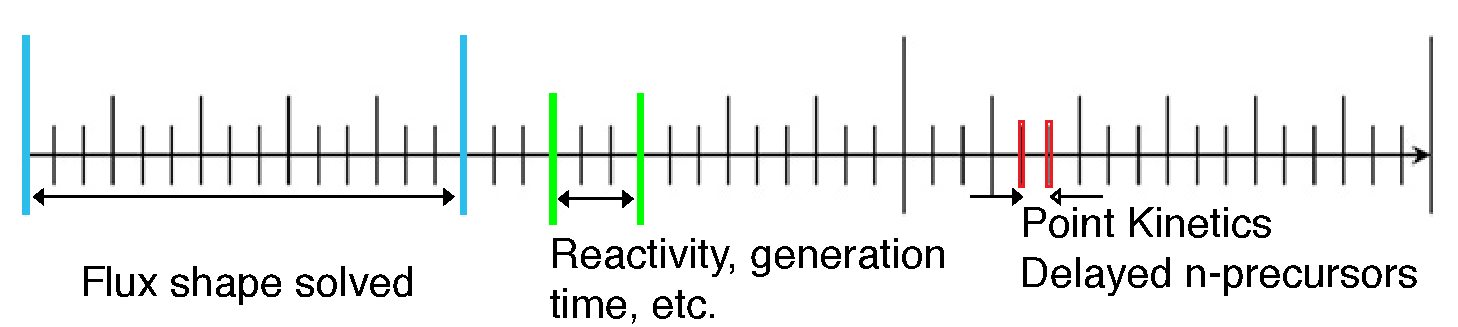
\includegraphics[width=8cm]{figures/time_scale.pdf}
    \caption{Time scale variation for IQS.}
    \label{fig:time_scale}
\end{figure}

The advantage of these varying time scales is computational savings.  This comes from the flux shape being solved on a large time steps and only done when the spatial distribution of neutrons changes significantly.  In between flux shapes the corresponding differential equations are solved to capture the time dependent behaviour.  Reactivity, generation time, and delayed neutron fraction are found from their inner product definitions and fed into the point kinetics equations.  Alternatively these values may be computed during the Monte Carlo random walk but required significant neutron histories to achieve low uncertainties (Waddell). In some IQS implementations there are tests to determine if the time step is too large to solve the flux shape over (Dulla). 

\begin{figure}[h]
    \centering
    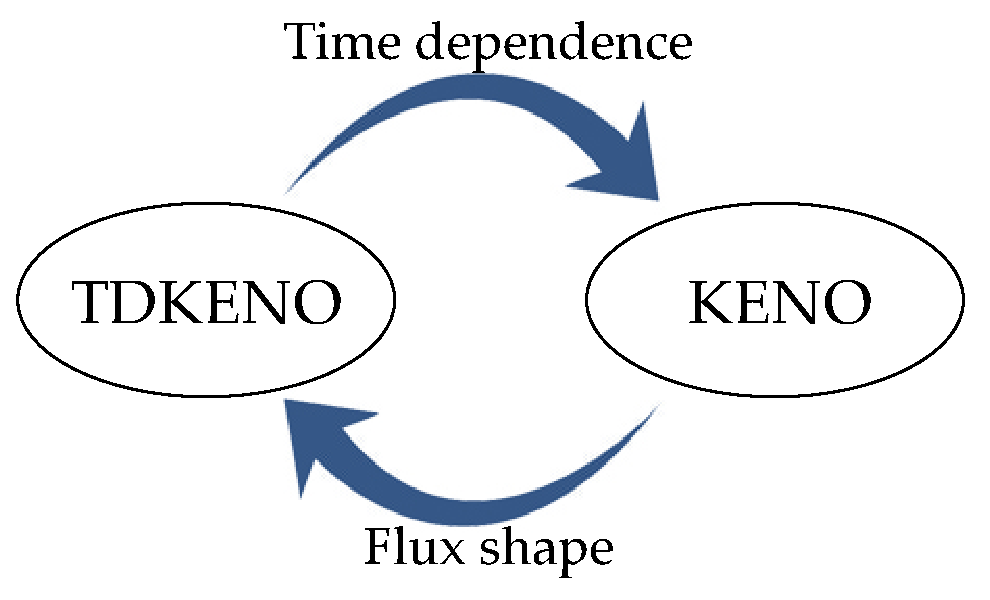
\includegraphics[width=7cm]{figures/tdkeno_flow.pdf}
    \caption{Relationship between TDKENO and KENO.  TDKENO drives the time dependence, getting the spatial neutron distribution from KENO.}
    \label{fig:tdkeno_flow}
\end{figure}

 In its current formulation, TDKENO does not do this but rather lets the user define when the a flux shape should be calculated.  This gives flexibility and may allow for computational savings as transients often experience a rapid change in neutron distribution and rapidly come to a steady state therefore not requiring a new calculation of the flux shape. However, since taking too large of a step is a possibility and may result in less quality answer, we are motivated to study the affects of varying the number of shape calculations prescribed.

%Equations look exceedingly pretty. Here is a 3-D, monoenergetic, steady-state
%transport equation with isotropic scattering and an isotropic extraneous source:
%\begin{subequations} \label{eqs:fullTransport}
%\begin{multline} \label{eq:fullTransportVol}
%  \vec{\Omega}\vd \grad \psi(\vec{x}, \vec{\Omega})
%  + \sigma(\vec{x}) \psi (\vec{x}, \vec{\Omega})
%\\ =
%  \frac{\sigma_s(\vec{x})}{4\pi} \int_{4\pi} \psi(\vec{x},\vec{\Omega}')
%  \ud\Omega' + \frac{q(\vec{x})}{4\pi}
%  \equiv \frac{1}{4\pi} Q(\vec{x}) \,,
%\end{multline}
%inside $\vec{x} \in V$, $\vec{\Omega} \in 4\pi$, with an incident boundary
%condition
%\begin{equation} \label{eq:fullTransportBndy}
%  \psi(\vec{x}, \vec{\Omega}) = \psi^b(\vec{x}, \vec{\Omega}) \,,
% \quad \vec{x} \in \partial V, \ \vec{\Omega} \vd \vec{n} < 0\,.
%\end{equation}
%\end{subequations}

%%%%%%%%%%%%%%%%%%%%%%%%%%%%%%%%%%%%%%%%%%%%%%%%%%%%%%%%%%%%%%%%%%%%%%%%%%%%%%%%
\section{Results and Analysis}
With the integration of the latest version of KENO from SCALE 6.2 we now have the ability to calculate the most intensive portion of the calculation in parallel.  Previously for problems with complex geometry the calculation of the shape may have taken several days to weeks when using to achieve adequate sampling and statistics.  By running TDKENO at the University of Florida's HiperGator supercomputer we are able to run on hundreds of CPUs resulting in the same calculations taking several hours.  These improvements are illustrated by comparing the time and memory usage with parallel KENO.  We apply these improvements to a particularly challenging problem of modeling the transients experiments with the Transient Reactor Test Facility (TREAT).



%%%%%%%%%%%%%%%%%%%%%%%%%%%%%%%%%%%%%%%%%%%%%%%%%%%%%%%%%%%%%%%%%%%%%%%%%%%%%%%%
\subsection{Computational Improvements}

\begin{table}[h]
    \centering
    \begin{tabular}{c|c|c}
                           & Memory & Cores \\
        KENO-VI (serial)   &        & 1 \\ 
        TDKENO             &        & 1  \\
        KENO-VI (parallel) &        & 40 \\
        TDKENO             &        & 1 \\
    \end{tabular}
    \caption{Caption}
    \label{tab:my_label}
\end{table}

%Later on, we can include a table, even one that spans two columns such as
%Table~\ref{tab:widetable}.
%%%%%%%%%%%%%%%%%%%%%%%%%%%%%%%%%%%%%%%%%
%\begin{table*}[htb]
%  \centering
%\begin{tabular}{llllllllll}\toprule
%      & $\phi_T(0)$      & $\phi_T(10)$      & $\phi_T(20)$      &
%      $\phi_D(0)$      & $\phi_D(10)$      & $\phi_D(20)$      & $\rho$      &
%      $\varepsilon$      & $N_\text{it}$
%\\ \midrule
%$c=0.999$  & 0.9038 & 20.63 & 31.24 & 0.9087 & 20.63 & 31.23 & 0.2192 & $10^{-7}$ & 15
%\\
%$c=0.990$  & 0.3675 & 13.04 & 24.7 & 0.3696 & 13.04 & 24.69 & 0.2184 & $10^{-7}$ & 15
%\\
%$c=0.900$  & 0.009909 & 4.776 & 17.64 & 0.009984 & 4.786 & 17.63 & 0.2118 & $10^{-7}$ & 14
%\\
%$c=0.500$  & $6.069\times 10^{-5}$ & 2.212 & 15.53 & 6.213$\times 10^{-5}$ & 2.239 & 15.53 & 0.2068 & $10^{-7}$ & 13
%\\
%\bottomrule
%\end{tabular}
%  \caption{This is an example of a really wide table which might not normally
%  fit in the document.}
%  \label{tab:widetable}
%\end{table*}
%%%%%%%%%%%%%%%%%%%%%%%%%%%%%%%%%%%%%%%%


%%%%%%%%%%%%%%%%%%%%%%%%%%%%%%%%%%%%%%%%%%%%%%%%%%%%%%%%%%%%%%%%%%%%%%%%%%%%%%%%
\subsection{TREAT Modeling}
M8CAL 2855 only?

\begin{table}[h]
    \centering
    \begin{tabular}{c|c|c}
         & TDKENO-K5 & TDKENO-K6 \\
        Generations &  10000 & 10000 \\
        Particles   &  10000 & 10000 \\
        Skipped     &  500   & 500  \\
    \end{tabular}
    \caption{Caption}
    \label{tab:my_label}
\end{table}

%%%%%%%%%%%%%%%%%%%%%%%%%%%%%%%%%%%%%%%%%%%%%%%%%%%%%%%%%%%%%%%%%%%%%%%%%%%%%%%%
\section{Conclusions}


%%%%%%%%%%%%%%%%%%%%%%%%%%%%%%%%%%%%%%%%%%%%%%%%%%%%%%%%%%%%%%%%%%%%%%%%%%%%%%%%
%\appendix
%\section{Appendix}
%
%Numbering in the appendix is different:
%\begin{equation} \label{eq:appendix}
%  2 + 2 = 5\,.
%\end{equation}
%and another equation:
%\begin{equation} \label{eq:appendix2}
%  a + b = c\,.
%\end{equation}

%%%%%%%%%%%%%%%%%%%%%%%%%%%%%%%%%%%%%%%%%%%%%%%%%%%%%%%%%%%%%%%%%%%%%%%%%%%%%%%%
\section{Acknowledgments}
This material is based upon work supported a Idaho National Laboratory.

%%%%%%%%%%%%%%%%%%%%%%%%%%%%%%%%%%%%%%%%%%%%%%%%%%%%%%%%%%%%%%%%%%%%%%%%%%%%%%%%
\bibliographystyle{ans}
\bibliography{bibliography}



\end{document}

